\documentclass[]{spie}  %>>> use for US letter paper
%\documentclass[a4paper]{spie}  %>>> use this instead for A4 paper
%\documentclass[nocompress]{spie}  %>>> to avoid compression of citations

\renewcommand{\baselinestretch}{1.0} % Change to 1.65 for double spacing
 
\usepackage{amsmath,amsfonts,amssymb}
\usepackage{graphicx}
\usepackage[colorlinks=true, allcolors=blue]{hyperref}

\title{Measuring Dark Energy and Radio Transients with HIRAX}

\author[a]{L.B. Newburgh}
\author[b]{Barry B. Author}
\affil[a]{Dunlap Institute, University of Toronto, 50 St. George St., Toronto, Canada}
\affil[b]{Affiliation2, Address, City, Country}

\authorinfo{Further author information: (Send correspondence to L.B.N.)\\L.B.N.: E-mail: newburgh@dunlap.utoronto.ca}

% Option to view page numbers
\pagestyle{empty} % change to \pagestyle{plain} for page numbers   
\setcounter{page}{301} % Set start page numbering at e.g. 301
 
\begin{document} 
\maketitle

\begin{abstract}
The Hydrogen Intensity and Real-time Analysis eXperiment (HIRAX) is a new 400--800\,MHz radio interferometer under development for deployment in South Africa. HIRAX will comprise 1024 6-m parabolic dishes on a compact grid, and the array will map most of the southern sky over the course of three years. HIRAX has two primary science goals: to constrain dark energy and measure structure at high redshift, and to study radio transients and pulsars. HIRAX will observe unresolved sources of neutral hydrogen via their redshifted 21-cm emission line (hydrogen intensity mapping), and the resulting maps of large scale structure at redshifts 0.8--2.5 will be used to measure baryon acoustic oscillations (BAO). BAO are a preferential length scale in the matter distribution that can be used to chart the expansion history of the universe and thus probe the nature of dark energy. HIRAX will improve upon current BAO measurements from galaxy surveys by observing a larger cosmological volume (both from increased survey area and redshift range) and also by measuring at high redshift when the expansion of the universe transitioned to dark energy-dominated. HIRAX will complement CHIME, a hydrogen intensity mapping effort in the northern hemisphere, by completing the sky coverage in the same redshift range. HIRAX's location in the Southern Hemisphere also allows a variety of crosscorrelation measurements with surveys of structure at many wavelengths. Daily maps of a few thousand square degrees of the Southern Hemisphere, encompassing the entire plane of the Milky Way galaxy, will also open new opportunities for discovering and monitoring radio transients. The HIRAX correlator will have the ability to rapidly and efficiently detect transient events; the results will shed light on the poorly understood nature of fast radio bursts (FRBs), enable pulsar monitoring to enhance long-wavelength gravitational wave searches, and provide a rich data set for searching for new radio transient phenomena. In this paper, we will discuss the HIRAX instrument, science goals, and current status.
\end{abstract}

% Include a list of keywords after the abstract 
\keywords{Cosmology, Dark Energy, Large Scale Structure, Intensity Mapping, 21cm}

\section{INTRODUCTION}
\label{sec:intro}  % \label{} allows reference to this section

Recent measurements from Type Ia supernovae (SN1a) [eg newest ref], baryon acoustic oscillations (BAO) [eg Eisenstein ref], and the cosmic microwave background (CMB) [eg Planck ref] have shown that the universe is dominated by dark energy, an unknown component that is causing the expansion rate of the universe to accelerate. To better understand the nature of dark energy, we require measurements around a redshift of $z\sim2$, when dark energy began to influence the rate of expansion.  For this task, BAO provide a powerful observational tool that can additionally be extended to higher redshifts.  BAO are characteristic scales in the matter power spectrum that are imprinted by primordial acoustic oscillations in the photon--baryon fluid at $z\sim 1100$.  The resulting characteristic comoving 150\,Mpc scale is present as a feature in the large scale structure distribution: structure forms preferentially with this length scale, and the physical length grows with the expansion of the universe. Measurements of the BAO length scale are thus sensitive tracers of the expansion rate of the universe, allowing us to probe dark energy and its evolution.  Recent galaxy surveys [recent BOSS ref] have already demonstrated percent-level constraints on dark energy at redshift $z\sim0.6$. \newline

A promising technique for measuring BAO at higher redshifts is 21-cm intensity mapping.  In this method, galaxies are observed in aggregate through low-resolution measurements of redshifted 21-cm emission of neutral hydrogen.  Neutral hydrogen is stored in galaxies, and the redshift is uniquely identified by the frequency of the measured 21-cm line emission.  Therefore, intensity mapping allows us to focus sensitivity on the large BAO scales of interest and trace the redshift evolution of that structure. The Hydrogen Intensity and Real-time Analysis eXperiment (HIRAX)\footnote{http:\//\//www.acru.ukzn.ac.za\//$\sim$hirax} is a new 400--800\,MHz radio interferometer that is under development in South Africa. HIRAX will map large scale structure in a redshift range of $0.8 < z < 2.5$ with 1024 6-m dishes. With southern sky coverage, HIRAX will complement CHIME [Kevin ref] in the Northern Hemisphere
% HCC: I commented out this sentence bit since it seems out of place in the general intro.  We should move it to a more instrumental section.
%and also leverage correlator technology development for CHIME [Nolan ref].
and will additionally take advantage of potential cross-correlations with wide-field surveys at other wavelengths (LSST, ACTPol, HST, DESI, DES, SPTpol). At minimum, cross-correlations with high-redshift galaxy surveys will provide an estimate for the neutral hydrogen bias and the neutral hydrogen fraction.

{\bf HCC: this last sentence seems a bit weak and doesn't really sell the crosscorrelation case.  Can we beef it up with another sentence or two, e.g. on foreground rejection and reduction of systematics?}
\newline

\textbf{Can we use Mario's/Amadeus's plots here? do we have any number for wa?}

 \begin{figure} [ht]
  \begin{center}
   \begin{tabular}{c} %% tabular useful for creating an array of images 
   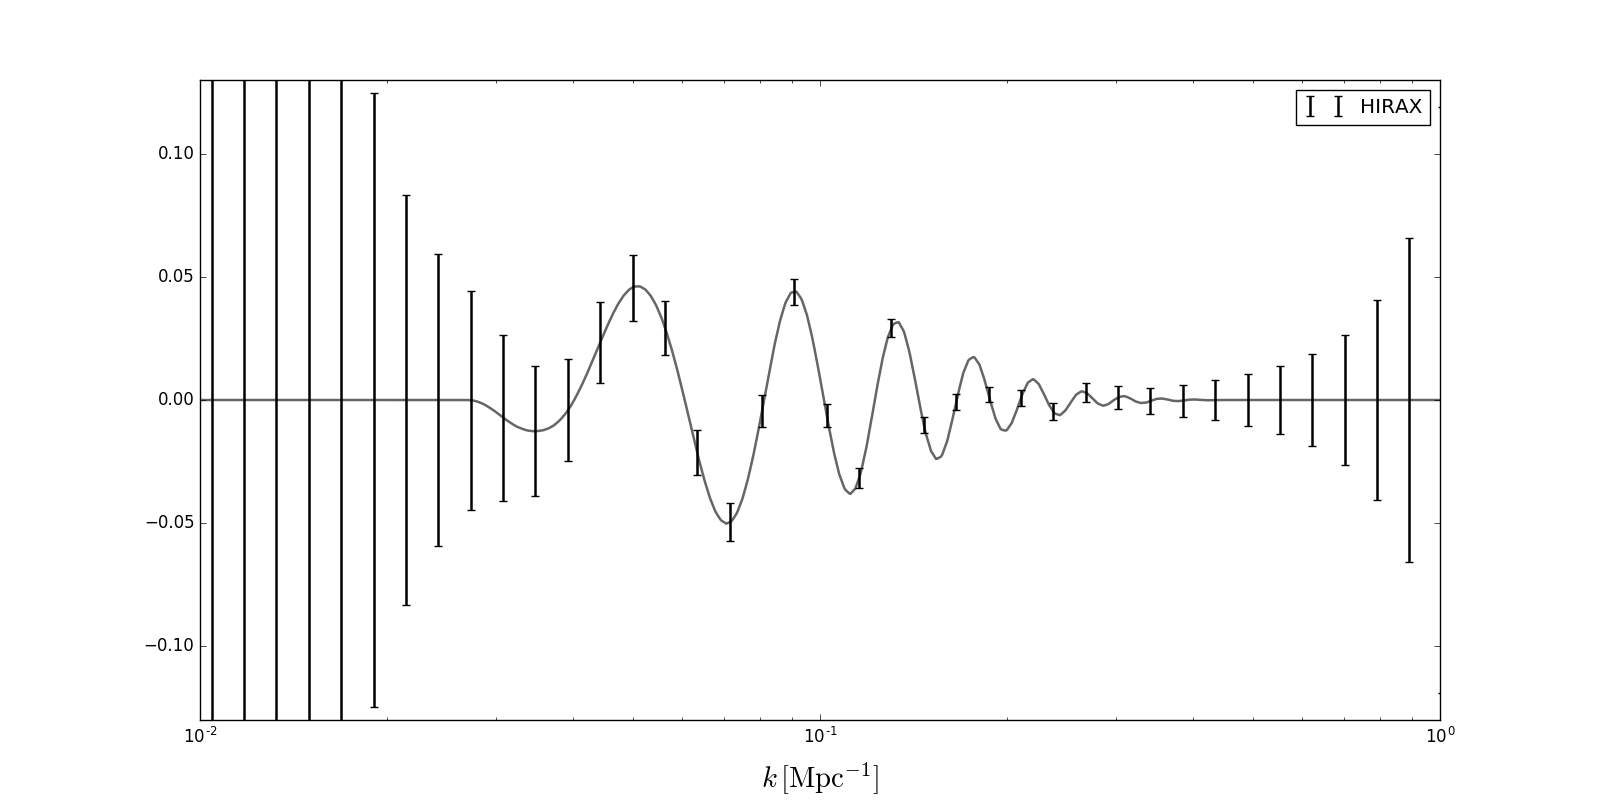
\includegraphics[height=5cm]{fbao_constraints_hirax.png}
   \end{tabular}
   \end{center}
   \caption[Power Spectra] 
%>>>> use \label inside caption to get Fig. number with \ref{}
   { \label{fig:pspec} 
Power spectra, credit Amadeus }
   \end{figure} 

  \begin{figure} [ht]
  \begin{center}
   \begin{tabular}{c} %% tabular useful for creating an array of images 
   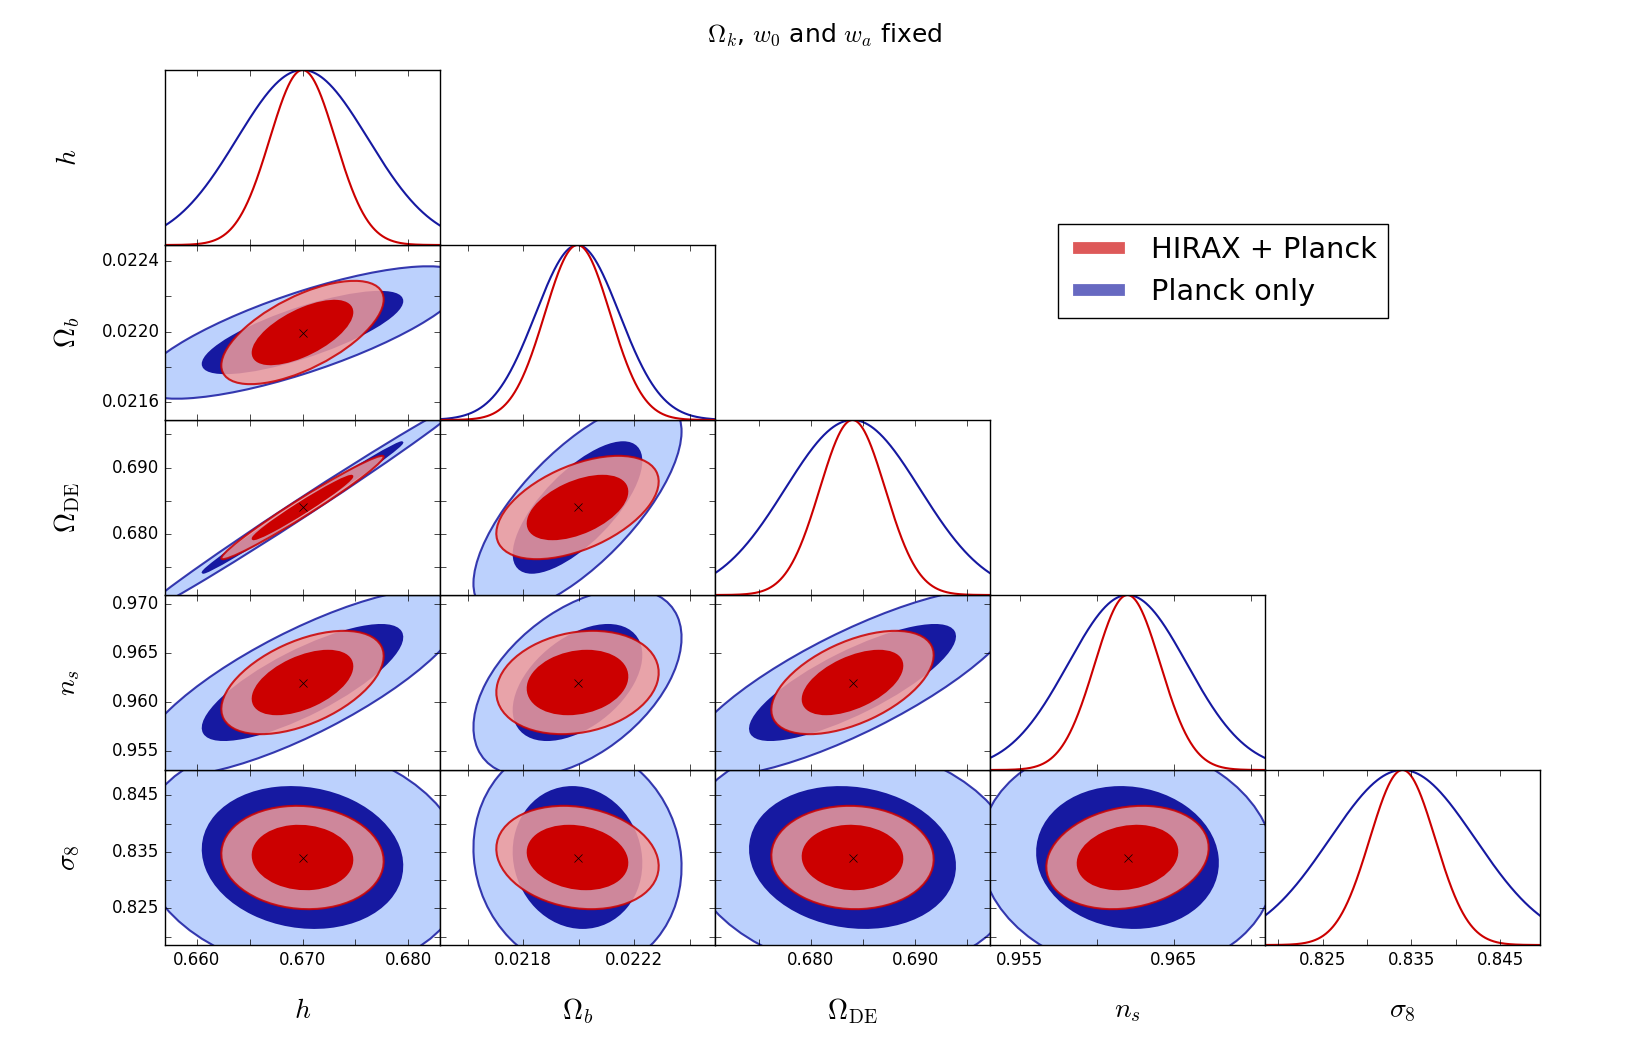
\includegraphics[height=5cm]{5pellipses_justHIRAX1.png}
   \end{tabular}
   \end{center}
   \caption[Contours] 
%>>>> use \label inside caption to get Fig. number with \ref{}
   { \label{fig:contours} 
Contours with lots of things held fixed, credit Amadeus}
   \end{figure} 


In addition to rich cross-correlation opportunities, observations of the southern sky will provides access to the entire Galactic plane, enabling a wide variety of transient measurements with HIRAX. Current and future observatories are studying the transient sky, with detection capabilities in the optical (LSST [ref]) and the new ability to detect gravitational waves with LIGO [ref]. HIRAX will add radio transient monitoring to this suite of observations and could be particularly useful for kilonova [ref]. In addition, Fast Radio Bursts (FRBs) are a source of enormous interest to the radio transient community because of their high dispersion measures and isotropic spatial distributions, indicating possible cosmological distances [ref]. Their origin is unknown and the subject of ongoing study [ref ref ref]. Projecting from current discovery rates of FRBs, HIRAX will find dozens per day (with significant uncertainty due to limited FRB statistics in the HIRAX band) and be able measure properties associated with their spectra, timing, and distribution. In addition to FRBs, HIRAX can be used as a pulsar discovery engine and to monitor pulsar times. The former will increase the number of known pulsars by \textbf{NN?}, and the latter daily monitoring would be a natural partner in pulsar timing arrays, which can potentially map long-wavelength gravity waves inaccessible to other probes. \newline 

Currently we are building an 8-element prototype array (HIRAX-8) at the Hartebeesthoek Radio Astronomical Observatory (HartRAO) to begin developing the analog system and analysis pipelines. After initial decisions on instrumentation informed by the prototype, we will build a 128-dish (HIRAX-128) instrument from which we will build out to the final 1024-dish HIRAX array (HIRAX-1024). {\bf HCC: move this paragraph to the instrument section?} \newline

In this paper we describe the instrument itself (Section~\ref{sec:instru}) including its reflector design, analog chain, and digitization; and some of the known challenges to this technique (Section~\ref{sec:chall}).


\section{The HIRAX Instrument}
\label{sec:instru}

The main driver for the HIRAX design is the measurement of large scale structure at high redshift. The redshift-dependent 150\,Mpc BAO feature ranges from 1.35$^{\circ}$ at z=2.5 (400\,MHz) to 3$^{\circ}$ at z=0.8 (800\,MHz). To sample the third acoustic peak at high redshift would require a baseline distance of at least 80\,m. To resolve the BAO feature along the line of sight (in the redshift direction), requires frequency resolution of at least 12\,MHz. The signal level is also small, $\mathcal{O}$(0.1\,mK), requiring low system noise and large collecting area. \newline 

The HIRAX instrument will be comprised of 1024 6\,m dishes deployed in a 32$\times$32 grid with the square sides aligned on the celestial cardinal directions. HIRAX is a transit telescope: the dishes will be pointed at a given declination, and the sky will rotate overhead in a constant drift-scan. Thus each pointing of the dishes will give us access to a $\sim6^{\circ}$ wide stripe of the sky. To map the entire sky, the dishes will be re-pointed once every 3 months, to complete a full 15,000$\mathrm{deg}^{2}$ survey (40\% of the sky) in $\sim$3 years. To map the sky to a depth of 1.2$\mu$Jy in 3 months requires a system noise of 40\,K \footnote {$\sigma_{Jy} = \frac{T_{sys} / R }{\sqrt{N_{dish} \Delta\nu \delta t N_{days}*t_{beam~crossing}}}$, where R[T/Jy] = $\frac{10^{-26}}{2k}A_{e}$, $A_{e}\sim1024*0.5*\pi*3^{2}$, and the beam crossing time is about 17\,mins. }. 
%Its location in the Karoo desert provides for protection from Radio-frequency interference (RFI) in the HIRAX bands. 
\newline

Each of the 1024 signal chains is composed of one radio dish, one antenna feed, two amplifiers (one per polarization), Radio-Frequency-over-Fiber (RFoF) to carry the signal to the correlator building, and the instrument correlator. These components are described below, the fiducial design has a target noise temperature of 50\,K, collecting area of $\sim29,000m^{2}$, for a daily sensitivity of $\sim 12 \mu$Jy/pixel. A few key design parameters for HIRAX-1024 are given in Table~\ref{tab:salient}.

\begin{table}[ht]
\caption{Instrument summary} 
\label{tab:salient}
\begin{center}       
\begin{tabular}{|l|l|} 
\hline
\rule[-1ex]{0pt}{3.5ex}  Frequency Range & 400--800\,MHz  \\
\hline
\rule[-1ex]{0pt}{3.5ex}  Frequency Resolution & 390\,kHz, 1024 bins \\
\hline
\rule[-1ex]{0pt}{3.5ex}  Dish size & 6\,m diameter, $f/D$=0.25 \\
\hline
\rule[-1ex]{0pt}{3.5ex}  Interferometric layout & 32$\times$32 square grid, 7\,m spacing  \\
\hline
\rule[-1ex]{0pt}{3.5ex}  Field of View & 15 deg$^{2}$--56 deg$^{2}$ \\
\hline
\rule[-1ex]{0pt}{3.5ex}  Resolution & $\sim$5'--10'  \\
\hline 
\rule[-1ex]{0pt}{3.5ex}  System Temperature & 50\,K   \\
\hline 
\end{tabular}
\end{center}
\end{table}


\subsection{Antennas: Dishes and Feeds}

The antennas for HIRAX are still under development, and include the dishes, the feed itself, a choke for the feed, and possibly active amplification built into the feed. The primary consideration is to have fast mapping speed, requiring high sensitivity. This in turn drives us to have a large collecting area and extremely efficient antennas: high aperture efficiency (60\%), low loss in the feed ($<-15$\,dB), a low reflection coefficient at the feed ($<-15$\,dB), and low spillover to the ground ($<10K$). \newline

\textit{Dishes --} The dishes will be approximately 6\,m diameter parabolic reflectors with an $f/D$ of 0.25. The small focal ratio will help cut down on crosstalk between neighboring antennas.  Because we image the sky in strips, changing the center declination every $\sim$3\,months, the dishes must be able to tilt on one axis. We have initial dish designs for the HIRAX-8 prototype array and are in the process of re-designing the dishes based on experiences in the field and with the vendor, in particular building rockers into the frame for full access to all of our target declinations. Any design must be cost efficient and easy to assemble, as well as have repeatable surface shaping and reflector surface imperfections constrained to $\frac{\lambda}{50}$ = 7\,mm [ref Ruze]. The dishes should also be rigid enough that the beam full-width-half-max does not change by more than $10^{-4}$ upon tilting up to 25$^{\circ}$. We would also like to minimize the reflections off of the support struts above the frame, for example by moving to a radio-transparent support. To reduce ground spillover and cross-talk, we are considering adding reflective collars to the dishes. \newline

%xxx where does 10^-4 come from?

\textit{Feeds -- } The HIRAX feed will be a modified version of the feed used for CHIME [Meiling ref], a dual-polarized clover-leaf shaped dipole antenna which has impressive characteristics across a wide band, which in turn was based on a four-square antenna developed for Molonglo [ref]. The feed is composed of: (i) a FR4-dielectric printed circuit board (PCB) which has four metalized curved petals on the front to act as an antenna, (ii) a low-loss teflon balun for impedance matching, and a teflon support board. The signal current distribution, design parameters, and beam characteristics are described in detail elsewhere [ref Kevin,ref Meiling], here I will note just that the shape of the petals provides sensitivity to a wide bandwith and there is one output signal for each linear polarization. \newline

The CHIME feed beam shape is designed for a cylindrical dish, and its impedance was chosen to minimize the noise of the low-noise amplifier at the feed output. For HIRAX, we would like circular beams with good impedance matching to the dish, and we are in the process of modifying the feed design accordingly. To circularize the beam and aid in reducing cross-talk and ground spill, we will be adding a ring choke structure, which will also help us weather-proof the instrumentation at the focus. Various choke ring geometries are being simulated to optimize gain, reduce spillover, and reduce polarization artifacts, where included in that optimization is the fact that while wider chokes are more effective at reducing spillover, they also increase the blockage of the center of the dish. \newline


\subsection{Amplification -- do we feel comfortable wtih a plot or picture of anything yet?}

To achieve fast mapping speeds, we are targetting a system noise of 50\,K. This will require not merely minimizing losses in the optical chain as described above, but also amplifying the signal either on or directly behind the feed with low noise amplifiers. The averaged sky signal is $\sim$50\,K %really?  I thought it was much lower
and we would like to digitize that signal such that its level on the input to the digitizer is-21\,dBm across the 400\,MHz bandwidth. The total input power from the average 50\,K sky would be -95\,dBm across the entire band, leading us to require about 75\,dB of total gain. As noted below, 50\,dB of that gain must come before the RFoF system for the system noise to be dominated by the LNA noise figure. We are investigating two routes for this amplification: including the amplification circuitry directly on the balun and backboard, and adding amplifiers attached at the SMA-connectorized outputs of the feeds. The benefits of amplifying directly on the feed is primarily a reduction in system noise by removing the connector, a source of loss between the feed and the first active stage amounting to an extra $\sim$3\,K in system noise. Whether we ultimately have amplifcation on the board or after a connector, we are currently planning to use Avago MGA-16116 GaAs MMIC low noise amplifiers, which have 0.37\,dB Noise Figure (25.8\,K) and $\sim$22\,dB gain, and so we will have to add additional amplification after this stage. \newline

To carry signals from the dishes to the correlator, radio interferometers and telescopes have traditionally used coaxial cable. However, optical fiber is an attractive solution for long cable runs when the loss (and its steep frequency dependence) can be prohibitive. The HIRAX array is large ($\sim$250\,m x 250\,m), and we are planning to use Radio-Frequency-over-Fiber (RFoF) to send the signals from the dish to the correlator building. The RFoF modules were developed for radio telescopes [ref] and have two parts: a transmitter at the dish and a receiver at the correlator building, with optical fiber in between. They have relatively high noise (typically 27\,dB ENR), and so must have at least 50\,dB of gain before the RFoF transmitter-receiver pair for the noise to be dominated by a front-stage LNA. The RFoF also contains the band-defining 400-800\,MHz filter and can be designed to have the final amplification stages required in the HIRAX signal chain. This RFoF system has been developed for radio telescopes in general, tested in the lab, and a prototype set was deployed and tested on CHIME. \newline      

\subsection{Digital Back End}

The HIRAX digital backend is an FX correlator, and will leverage development for the correlator for CHIME. The correlator architecture and implementation has been described thoroughly in [ref, ref, ref], so here I will merely describe the general data processing steps. The F-engine performs frequency channelization using a set of custom boards, each of which takes 16 sky channels. For HIRAX-8 we can use just one board, for HIRAX-128 we will require 16 boards, and for HIRAX-1024 we will require 128 boards. The signal from each input is digitized at 8-bit precision at 800\,MHz. The signal is then sent through a customized poly-phase filter bank (PFB) and FFT algorithm, performed at 16-bit precision, developed from CASPER [ref] to channelize the signal into 1024 frequency channels between 400--800\,MHz. The X-engine of the correlator will correlate all sky inputs for each of the 1024 frequency channels, and is implemented in an array of GPU nodes. To transfer the data between the FPGA F-engine and the GPU X-engine, the data is sent on a custom backplane which performs the quarter turn operation. The quarter takes the output from the FPGA, which is natively 1024 frequency channels for each sky input, and re-arranges and shuffles them into the format required for the X-engine, namely all sky inputs for a single frequency. \newline

The quarter-turned data is sent to the GPU X-engine on 10\,Gbps lines. The diskless nodes will contain two network cards and two to four GPUs (depending on models selected), and the GPUs run a custom kernel to efficiently calculate the per-frequency correlation matrix. Each GPU correlator node is responsible for 32/4 frequency channels for all sky inputs for HIRAX-128/full HIRAX. The data is accumulated and written to a separate storage system. \newline

The correlator will also form tied-array beams across the primary beam to search for transients, pulsars, hydrogen absorbers, and the like.  The antenna locations on a regular grid simplifies beamforming.  This can be done either via FFTs or direct summation which scales like $n^{3/2}$ instead of $n^2$ for regularly-spaced antennas in two dimensions.  The frequency resolution of the formed beams will be increased by a factor of 32, which can be done by approximately inverting the polyphase filter bank in the correlator.  These formed beams will be searched for FRBs using tree algorithms [ref Masui et al.], and a subset of approximately 20 beams will be passed to a pulsar search engine.


\subsection{Current Status}

We are currently building HIRAX-8, a prototype array of 8 dishes, at Hartebeesthoek Radio Astronomical Observatory (HartRAO), located $\sim$ 100\,km outside of Johannesburg. From an RFI perspective, its proximity to Johannesburg is not ideal (and so the full HIRAX array will not be deployed there), however it is easy to access and has a variety of resources which make it a useful site for building a small prototype array. The prototype dishes have been ordered, and some initial instrumentation has already been deployed on commercial dishes. HIRAX-8 will have 16 total inputs (two polarizations from each of the 8 dishes), for which we can use one FPGA board and an off-the-shelf computer for correlation and data storage. The correlator is in a faraday cage at HartRAO and we are currently building up to continuous operations with the small commercial dishes. When the prototype dishes arrive, we will upgrade the array to its full 8 elements, and continue using the array to test newly developed hardware until we have a stable design. At that point we will build the 128-dish HIRAX-128, with 256 inputs. HIRAX-8 and HIRAX-128 are currently funded, and will provide 3 $\times$ the collecting area already available on CHIME. %xxx should be clear this is chime pathfinder


\section{Foreground Removal Challenges}
\label{sec:chall}

The biggest challenge for all 21\,cm intensity mapping experiments is the presence of bright synchrotron foregrounds from our own Milky Way galaxy, which can be as bright as 700\,K. In theory these can be filtered due to their smooth spectral structure, as demonstrated in [ref]. As described in that paper, this removal hinges on the precise calibration of the instrument, primarily its beam (to 0.1\%) and its gain (to 1\%). This foreground filtering degrades our ability to measure large scale modes along the line of sight (because we filter smoothly in frequency), however it does not impact our ability to measure the matter power spectrum, which has features on smaller scales. \newline

The current plan for calibrating the beam is to use a drone-based beam measurement technique. We will fly a broad-band antenna and source on a quadcopter drone in a known pattern to map out the near field beams, and extrapolate to the far field (or measure the far field directly, when possible). Using drones for beam mapping has been previous demonstrated [ref] and multiple groups are pursuing this method of beam calibration at a variety of wavelengths. The far field of the HIRAX 6\,m dishes will be 96--192\,m across the band, which is within range of commercially available drones. We are currently buiding up the drone measurement program, with testing starting this year.\newline

We have chosen to place the HIRAX dishes on a grid to allow for maximum redundancy in baseline distances. Ultimately, this is to take advantage of redundancy for time-dependent gain calibration, as well as possible solutions for beam differences. The algorithm we are developing for HIRAX [ref sievers in prep] differs from traditional redundant calibration [ref liu] by using knowledge of the sky (whose prior can be incomplete and consist of basically just known bright point sources) to solve for gains only, using the expected visibility-visibility correlation function. This scheme allows the user to use knowledge of the array non-idealities and partial sky knowledge (in particular known positions of bright sources) to calibrate instrument gains and verify/possibly extract beam shapes. \newline

\section{Conclusion}

HIRAX is a radio interferometer designed to measure 15,000 $\mathrm{deg}^{2}$ of the sky to a depth of 1.2$\mu$Jy. The resulting maps of neutral hydrogen in 1024 frequency bins between 400--800\,MHz will provide low-resolution measurements of large scale structure to better understand the nature of dark energy through its impact on the expansion rate of the universe. HIRAX will also monitor the sky for radio transients, both fast irregular bursts (such as FRBs) and pulsars. The prototpye array, HIRAX-8, will be constructed this year at HartRAO and be used to finalize the design for the full instrument.

\label{sec:conc}



 %  \begin{figure} [ht]
  % \begin{center}
 %  \begin{tabular}{c} %% tabular useful for creating an array of images 
%   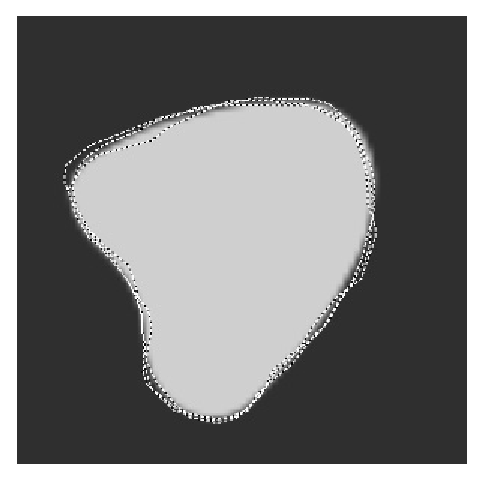
\includegraphics[height=5cm]{mcr3b.eps}
%   \end{tabular}
%   \end{center}
%   \caption[example] 
%%>>>> use \label inside caption to get Fig. number with \ref{}
%   { \label{fig:example} 
%Figure captions are used to describe the figure and help the reader understand it's significance.  The caption should be centered underneath the figure and set in 9-point font.  It is preferable for figures and tables to be placed at the top or bottom of the page. LaTeX tends to adhere to this standard.}
%   \end{figure} 
   

\acknowledgments % equivalent to \section*{ACKNOWLEDGMENTS}       
 
????

% References
\bibliography{report} % bibliography data in report.bib
\bibliographystyle{spiebib} % makes bibtex use spiebib.bst

\end{document} 
